\subsection{运动学}
\begin{tabularx}{\columnwidth}{XX}
  \multicolumn{2}{l}{\textbf{基本概念}}                                   \\
  瞬时速度            & $v=\lim\limits_{t\to0} \frac{\Delta x}{\Delta t}$ \\
  平均速度            & $v=\frac{\Delta x}{\Delta t}$                     \\
  瞬时速率            & $v=$瞬时速度大小                                        \\
  平均速率            & $v=\frac{\text{路程}}{\Delta t}$                    \\
  平均加速度           & $a=\frac{\Delta v}{\Delta t}$                     \\
  \multicolumn{2}{l}{\textbf{匀变速直线运动}}                                \\
  位移              & $x=v_0t+\frac{1}{2}at^2$                          \\
                  & $x=\frac{v_0+v}{2}t$                              \\
  速度              & $v=v_0+at=v_tt-at$                                \\
  速度平方            & $v^2=v_0^2+2ax$                                   \\
  中间位移速度          & $v=\sqrt{\frac{x_1^2+x_2^2}2}$                    \\
  中间时刻速度          & $v=\frac{x_1+x_2}{2}$                             \\
  相邻相等时间间隔位移差     & $\Delta x=aT^2$                                   \\
  第M段与第N段Ts时间内位移差 & $(M-N)aT^2$                                       \\
  \multicolumn{2}{l}{\textbf{从静止开始加速}}                                \\
  相等时间每段位移比       & $1:3:5:\cdots:2n-1$                               \\
  相等时间总计位移比       & $1:4:9:\cdots:n^2$                                \\
  相等位移间隔每段用时比     & $1:\sqrt2-1:\cdots:\sqrt n-\sqrt{n-1}$            \\
  相等位移间隔总计用时比     & $1:\sqrt2:\cdots:\sqrt n$                         \\
\end{tabularx}
\hfill
\begin{minipage}{0.48\columnwidth}
  \centering
  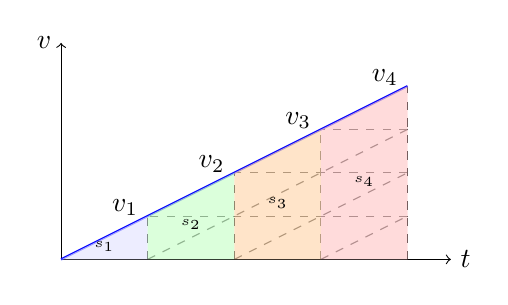
\begin{tikzpicture}[scale=1.1]
    % 坐标轴
    \draw[->] (0,0) -- (0,2.5) node[left] {$v$};
    \draw[->] (0,0) -- (4.5,0) node[right] {$t$};
    % 等时间间隔
    \foreach \i in {1,2,3,4}
    \draw[dashed] (\i,0) -- (\i,\i*0.5);
    \foreach \i in {1,2,3}
    \draw[dashed] (4,\i*0.5) -- (\i,\i*0.5);
    \foreach \i in {1,2,3}
    \draw[dashed] (\i,0) -- (4,2-\i*0.5);
    % 匀加速直线
    \draw[thick,blue] (0,0) -- (4,2);
    % 速度标记
    \foreach \i/\v in {0/1,1/2,2/3,3/4}
    \node[left] at (\i+1,\i*0.5+0.6) {$v_{\the\numexpr\i+1}$};
    \foreach \i/\col in {0/blue!10, 1/green!20, 2/orange!30, 3/red!20} {
        \fill[\col,opacity=0.7] (\i,0) -- (\i+1,0) -- (\i+1,\i*0.5+0.5) -- (\i,\i*0.5);
        \node at (\i+0.5,\i*0.25+0.15) {\tiny $s_{\the\numexpr\i+1}$};
      }
  \end{tikzpicture}
\end{minipage}
\hfill
\begin{minipage}{0.48\columnwidth}
  \centering
  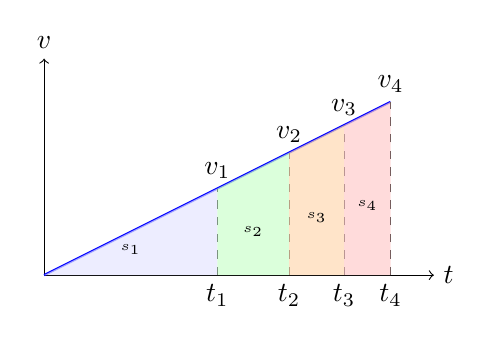
\begin{tikzpicture}[scale=1.1]
    % 坐标轴
    \draw[->] (0,0) -- (0,2.5) node[above] {$v$};
    \draw[->] (0,0) -- (4.5,0) node[right] {$t$};
    % 匀加速直线
    \draw[thick,blue] (0,0) -- (4,2);
    % 等位移间隔
    \foreach \i in {1,2,3,4}
    \draw[dashed] ({2*sqrt(\i)},0) -- ({2*sqrt(\i)},{sqrt(\i)});
    % 时间标记
    \node[below] at (2,0) {$t_1$};
    \node[below] at ({2*sqrt(2)},0) {$t_2$};
    \node[below] at ({2*sqrt(3)},0) {$t_3$};
    \node[below] at ({2*sqrt(4)},0) {$t_4$};
    % % 位移阴影
    \foreach \i/\col in {1/blue!10, 2/green!20, 3/orange!30, 4/red!20} {
        \fill[\col,opacity=0.7] ({2*sqrt(\i-1)},0) -- ({2*sqrt(\i)},0) -- ({2*sqrt(\i)},{sqrt(\i)}) -- ({2*sqrt(\i-1)},{sqrt(\i-1)});
        \node at ({(sqrt(\i)+sqrt(\i-1))},{sqrt(\i)*0.5-0.2}) {\tiny $s_{\the\numexpr\i}$};
      }
    \foreach \i in {1,2,3,4}
    \node[above] at ({2*sqrt(\i)},{sqrt(\i)}) {$v_{\the\numexpr\i}$};
  \end{tikzpicture}
\end{minipage}

\begin{formulanotebox}
  匀变速公式（如 $x=v_0t+\frac{1}{2}at^2$、$v=v_0+at$、$v^2=v_0^2+2ax$）仅适用于\textbf{加速度恒定}的一维直线运动，使用前先判断研究过程是否为同一段匀变速过程。

  “中间位移速度”“中间时刻速度”以及“相等时间/相等位移间隔比值”都建立在\textbf{从静止出发且做匀加速直线运动}的条件下，非此条件不可直接套用。
\end{formulanotebox}

\begin{keypointbox}
  \textbf{位移、路程与速度概念区分}：平均速度由位移决定，平均速率由路程决定，往返运动中两者通常不相等。单向直线运动中，位移大小等于路程。

  \textbf{图像物理意义}：\\
  $v$-$t$ 图像斜率表示加速度，图线与时间轴围成的面积表示位移；判断“加速/减速”要结合速度方向与加速度方向，而非只看速度大小变化。
  \text{x-t}图像切线斜率表示速度，图像零点表示初始位置，图像极值点表示运动反向点。
  \vspace{1em}
  \begin{center}
    \begin{tikzpicture}[scale=0.85]
      % 坐标轴
      \draw[->] (0,0) -- (5.2,0) node[right] {$t$};
      \draw[->] (0,-1.2) -- (0,2.6) node[above] {$x$};
      % x-t 曲线（抛物线，有极大值点）
      \draw[thick,blue,domain=0:4,samples=100,smooth] plot(\x,{2-0.6*(\x-2)^2});
      % 极大值点标记
      \filldraw[red] (2,2) circle (1.8pt);
      \node[above right,red] at (2,2) {反向点};
      % x轴和t轴刻度
      \foreach \x in {1,2,3,4}
      \draw (\x,0.07) -- (\x,-0.07) node[below] {$\x$};
      \foreach \y in {1,2}
      \draw (0.1,\y) -- (-0.1,\y) node[left] {$\y$};
      \draw[dashed,gray!70] (2,0) -- (2,2);
      \draw[dashed,gray!70] (0,2) -- (2,2);
    \end{tikzpicture}
  \end{center}
  \text{v-t}图像切线斜率表示加速度，图像的零点并且左右如果正负不同，那么这就是运动反向点。图像的极值点表示加速度为0，是最大或者最小值。图像与时间轴围成的面积表示位移，面积在时间轴上方表示正向位移，面积在时间轴下方表示反向位移。\\
  \begin{center}
    \begin{tikzpicture}[scale=0.85]
      % 坐标轴
      \draw[->] (0,0) -- (3.2,0) node[right] {$t$};
      \draw[->] (0,-0.9) -- (0,2) node[above] {$v$};
      % 抛物线曲线 v = -(t-2)^2 + 2
      \draw[thick,blue,domain=0.2:3.0,samples=100,smooth] plot(\x, {-(\x-1.5)*(\x-1.5)+1.4});
      % 极大值点 (1.5,1.4)
      \filldraw[red] (1.5,1.4) circle (1.7pt);
      \draw[red,thick,->] (1.5,1.65) -- (1.5,1.47);
      \node[red,above] at (1.5,1.68) {速度最大点};
      % 零点 (0.29,0) 和 (2.71,0)
      \filldraw[orange] (0.29,0) circle (1.5pt);
      \draw[orange,thick,->] (0.29,-0.33) -- (0.29,0.08);
      \node[orange,below] at (0.29,-0.33) {速度反向点};
      % t轴和v轴刻度
      \foreach \x in {1,2,3}
      \draw (\x,0.07) -- (\x,-0.07) node[below] {$\x$};
      \foreach \y in {1}
      \draw (0.08,\y) -- (-0.08,\y) node[left] {$\y$};
    \end{tikzpicture}
  \end{center}
  \text{a-t}图像与时间轴围成的面积表示速度变化量。图像在时间轴上方，那么面积认为是正的，否则就是负的，正的面积代表速度变化量为正。零点并且左右正负不同，该点为合力反向点，同时是速度的极值点，可能是极大值也可能是极小值，取决于左侧图像正与负，左侧为正，则该点为速度最大点，左侧为负，则该点为速度最小点。图像的极值点为加速度最大或者最小值。高中阶段无其他用处。
  \begin{center}
    \begin{tikzpicture}[scale=0.75]
      % 坐标轴
      \draw[->] (0,0) -- (3.2,0) node[right] {$t$};
      \draw[->] (0,-1.1) -- (0,1.6) node[above] {$a$};
      % a-t 曲线（正负对称穿过零点的正弦曲线）
      \draw[thick,blue,domain=0:3,samples=100,smooth] plot(\x, {1.2*sin(150*(\x-1.5))});
      % 零点 (1.5,0)
      \filldraw[red] (1.5,0) circle (1.7pt);
      \draw[red,thick,->] (1.5,0.35) -- (1.5,0.08);
      \node[red,above] at (1.5,0.36) {速度极值点};
      % t轴和a轴刻度
      \foreach \x in {1,2,3}
      \draw (\x,0.07) -- (\x,-0.07) node[below] {$\x$};
      \foreach \y in {1}
      \draw (0.08,\y) -- (-0.08,\y) node[left] {$\y$};
    \end{tikzpicture}
  \end{center}
\end{keypointbox}

\begin{casetypebox}
  [title={\strut\textcolor{white}{\bfseries 常见题型：自由落体}}]
  忽略空气阻力时，自由落体是初速度为零、加速度为 $g$ 的匀加速直线运动。

  \begin{center}
    \begin{tabular}{cc}
      \begin{minipage}{0.42\textwidth}
        \[
          \left\{
          \begin{aligned}
            v   & = gt               \\
            h   & = \dfrac{1}{2}gt^2 \\
            v^2 & = 2gh
          \end{aligned}
          \right.
        \]
      \end{minipage}
       &
      \begin{minipage}{0.50\textwidth}
        \begin{center}
          \begin{tikzpicture}[scale=1]
            % 坐标轴
            \draw[->] (0,0) -- (3.3,0) node[right] {$t$};
            \draw[->] (0,0) -- (0,3.0) node[above] {$v$};
            % v-t 线性上升（自由落体：v = gt, 初速度为0，向下为正）
            \draw[thick,blue] (0,0) -- (3,2.5);
            % 标点 (3,2.5)
            \filldraw[red] (3,2.5) circle (1.3pt);
            % 标注初速度为零
            \node[left] at (0,0) {0};
            % y轴刻度
            \draw (0,2.5) -- (0.10,2.5) node[right] {$gt$};
            % x轴刻度
            \draw (3,0.07) -- (3,-0.07) node[below] {$t$};
          \end{tikzpicture}
        \end{center}
      \end{minipage}
    \end{tabular}
  \end{center}

  自由落体由于是初速度为0的匀加速直线运动，所以之前的大量推论都可直接套用。这也是自由落体运动最喜欢考察的原因。
\end{casetypebox}

\begin{casetypebox}[title={\strut\textcolor{white}{\bfseries 常见题型：竖直上抛}}]
  竖直上抛可分为“上升减速”和“下降加速”两个阶段，且全程加速度恒为 $g$（方向竖直向下）。解题时优先统一坐标方向并分段列式，或直接用全程匀变速公式处理。

  \begin{center}
    \begin{tabular}{cc}
      \begin{minipage}{0.42\textwidth}
        \[
          \left\{
          \begin{aligned}
            h_\mathrm{max} & = \frac{v_0^2}{2g} \\
            t_0            & = \frac{v_0}{g}
          \end{aligned}
          \right.
        \]
      \end{minipage}
       &
      \begin{minipage}{0.50\textwidth}
        \begin{center}
          \begin{tikzpicture}[scale=1.09]
            \draw[->] (-0.1,0) -- (3.1,0) node[right] {$t$};
            \draw[->] (0,-1.3) -- (0,1.65) node[above] {$v$};
            \draw[dashed,gray] (0,0) -- (3.0,0);
            \draw[thick,blue,domain=0:3.0] plot(\x,{1.2-0.57*\x});
            \filldraw[red] (0,1.2) circle (1.13pt);
            \node[left] at (0,1.2) {$v_0$};
            \filldraw[red] ({1.2/0.57},0) circle (1.13pt);
            \node[below] at ({1.2/0.57},0) {$t_0$};
          \end{tikzpicture}
        \end{center}
      \end{minipage}
    \end{tabular}
  \end{center}

  虽然这是重力相关的竖直上抛，但是他的结论与刹车问题是一样的，刹车问题特别的地方是，如果是现实问题，汽车一般认为不能可以反向加速。
\end{casetypebox}

\begin{casetypebox}[title={\strut\textcolor{white}{\bfseries 常见题型：追击相遇问题（大追小）}}]
  追击相遇问题可以分成两类，加速度大的追加速度小的。加速度小的追加速度大的。
  初速度可以有区别，追赶就暗含了两者的初始位置关系。追击相遇问题可以采用图像法，也可以采用代数法。两种方法都会演示一遍。
  \text{注意}现实中如果并非追及而是碰撞，那么只能碰撞一次。也就是最近的一次，另一个解舍去。
  首先是加速度大的追加速度小的。
  \begin{center}
    \begin{tabular}{cc}
      \begin{minipage}{0.48\textwidth}
        \begin{center}
          \begin{tikzpicture}[scale=0.72]
            \draw[->] (-3,0) -- (5,0) node[right] {$t$};
            \draw[->] (0,-2) -- (0,4) node[left] {$v$};
            \draw[thick,blue,domain=-3:4] plot(\x,{0.0+0.45*\x});
            \draw[thick,red,dashed,domain=-3:3] plot(\x,{1.0+0.85*\x});
            \draw[dashed,gray] (4.2,0) -- (4.2,1.2);
            \draw[thick,black] (6.0,2.0) -- (6.4,2.0) node[right,black] {前};
            \draw[thick,black,dashed] (6.0,1.55) -- (6.4,1.55) node[right,black] {后};
          \end{tikzpicture}
        \end{center}
      \end{minipage}
       &
      \begin{minipage}{0.48\textwidth}
        \begin{center}
          \begin{tikzpicture}[scale=0.72]
            \draw[->] (0,0) -- (6,0) node[right] {$t$};
            \draw[->] (0,0) -- (0,5.2) node[left] {$v$};
            \draw[thick,blue,domain=0:6] plot(\x,{1.2+0.45*\x});
            \draw[thick,red,dashed,domain=0:6] plot(\x,{0.0+0.85*\x});
            \draw[dashed,gray] (3,0) -- (3,2.55);
            \filldraw[red] (3,2.55) circle (1.15pt);
            \node[below] at (3,0) {$t_0$};
            \draw[dashed,gray] (4.8,0) -- (4.8,1.2);
            \draw[thick,black] (6,2.0) -- (6.4,2.0) node[right,black] {前};
            \draw[thick,black,dashed] (6,1.55) -- (6.4,1.55) node[right,black] {后};
          \end{tikzpicture}
        \end{center}
      \end{minipage}
    \end{tabular}
  \end{center}

  你会注意到其实上面的两个图像其实只是初始位置不同，其他都是一样的。左侧是右侧的交点右侧图像而已。
  右侧图像说明开头两者之间距离增大，在$t_0$时候速度相等，距离达到最大。接着距离缩短，在某个时间达到相遇。
  左侧图像是速度相等的右侧部分，所以两者距离直接缩短，在某时刻相遇。

  接着对右图绘制一个相距距离图像，并且设初始距离为$d_0$，下面绘制图像：

  \begin{center}
    \begin{tikzpicture}[scale=0.82]
      \draw[->] (0,0) -- (5.6,0) node[right] {$t$};
      \draw[->] (0,-0.6) -- (0,3.8) node[left] {$\Delta x$};
      \draw[dashed,gray] (0,0) -- (5.4,0);

      % 相距距离：先增大后减小，过零时相遇
      \draw[thick,blue,domain=0:4.25,samples=120] plot(\x,{2+1.2*\x-0.4*\x*\x});

      % 初始距离 d0
      \draw[dashed,gray] (0,2) -- (0.55,2);
      \node[left] at (0,2) {$d_0$};
      \filldraw[blue] (0,2) circle (1.2pt);

      % 极值点 t0（速度相等时）
      \draw[dashed,gray] (1.5,0) -- (1.5,2.9);
      \filldraw[red] (1.5,2.9) circle (1.15pt);
      \node[below] at (1.5,0) {$t_0$};

      % 零点：相遇时刻
      \filldraw[red] (4.25,0) circle (1.15pt);
      \node[below right] at (4.25,0) {相遇时刻};
    \end{tikzpicture}
  \end{center}

  先设初速度差为$\Delta v$，加速度差为$\Delta a$，初始距离为$d_0$，相遇时刻为$t_0$。\\
  如果你想要用下面的公式，请严格按照，后方物体减前方物体的顺序，并且正负号带好。
  首先是速度相等点：
  \[
    t_0=\frac{\Delta v}{\Delta a}
  \]
  此时距离最大：
  \[
    x=\frac{\Delta v^2}{2\Delta a}+d_0
  \]
  相遇时刻为$t$：
  \[
    d_0=\Delta v t+\frac{1}{2}\Delta a t^2
  \]
\end{casetypebox}

\begin{casetypebox}[title={\strut\textcolor{white}{\bfseries 常见题型：追击相遇问题（小追大）}}]
  最后是另一种，加速度小的追及加速度大的物体，此时如果加速度小的物体初速度也小，那么一定无法追上，所以必须要初速度大于另一个物体。而且也还是有可能无法追上。
  \begin{center}
    \begin{tikzpicture}[scale=0.78]
      \draw[->] (0,0) -- (8.3,0) node[right] {$t$};
      \draw[->] (0,0) -- (0,4.3) node[left] {$v$};

      % 初速度大、加速度小（追）
      \draw[thick,blue] (0,1) -- (8,3);
      % 初速度小、加速度大（被追）
      \draw[thick,red,dashed] (0,0) -- (8,4);

      % 速度相等时刻 t0（两条 v-t 线交点）
      \draw[dashed,gray] (4,0) -- (4,2);
      \filldraw[red] (4,2) circle (1.15pt);
      \node[below] at (4,0) {$t_0$};

      % t0 左右两侧：两种可能的追及相遇时刻
      \draw[dashed,gray] (2,0) -- (2,1.2);
      \draw[dashed,gray] (6,0) -- (6,1.2);
    \end{tikzpicture}
  \end{center}
  存在一个速度相等点，此时两者的唯一达到最近，如果在该点无法相遇，那么就不可能相遇。
  相对的也可能在这之前就已经相遇了，如果能够多次相遇，那么会在关于速度相等点对称的时刻再次相遇。\\
  注意，下方的$\Delta v$与$\Delta a$都是后方减去前方，保留正负号。\\
  速度相等时间：
  \[
    t_0=\frac{\Delta v}{\Delta a}
  \]
  此时最短位移：
  \[
    x=\Delta v t_0+\frac{1}{2}\Delta a t_0^2-d_0
  \]
  如果能够相遇，那么一定存在：
  \[
    x\leq d_0
  \]
  相遇时间$t$时有：
  \[
    \Delta v t+\frac{1}{2}\Delta a t^2=d_0
  \]
  该方程有两个解。刹车问题一般取更小的合理解。

\end{casetypebox}
